\textbf{Model uczony na stałej krzywiźnie wierzechołków}

\begin{figure}[ht]
	\centering
	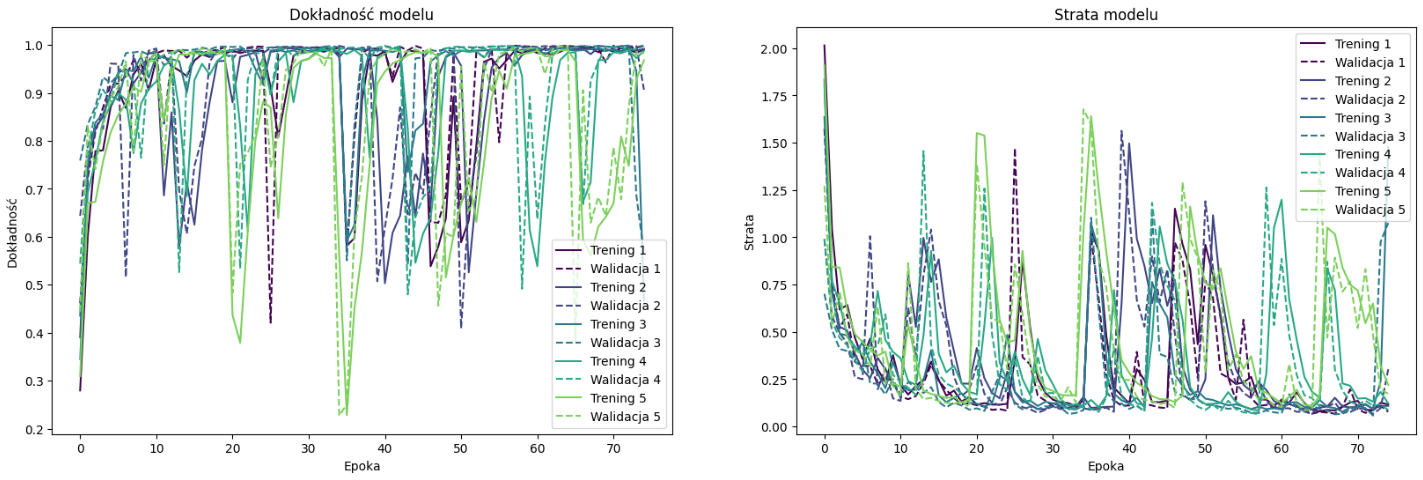
\includegraphics[height=5.5cm]{resources/tests/images/v2/crossvalid_img.png}
	\caption{Wyniki testów dla modelu z walidacją krzyżową i stałą krzywizną wierzechołków}
	\label{Fig:tests-cv-1}
\end{figure}
\FloatBarrier

\begin{figure}[ht]
	\centering
	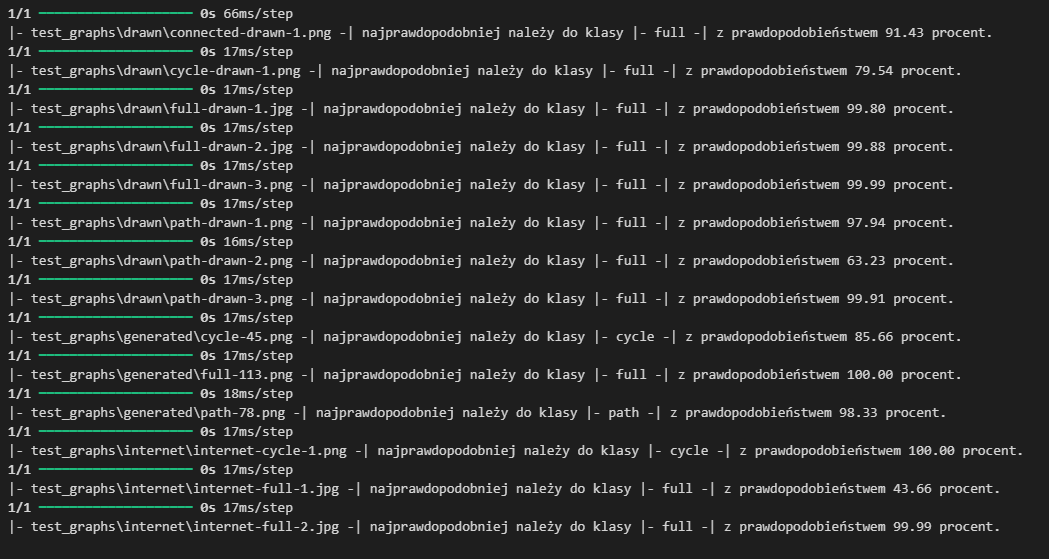
\includegraphics[height=7cm]{resources/tests/images/v2/crossvalid_txt.png}
	\caption{Klasyfikacja obrazów zewnętrznych dla modelu z walidacją krzyżową i stałą krzywizną wierzechołków}
	\label{Fig:tests-cv-2}
\end{figure}
\FloatBarrier

\textbf{Model uczony na losowej krzywiźnie wierzechołków}

W przypadku modelu z walidacją krzyżową, uczonego na grafach z 4 wierzchołkami,
dokładność wzrasta gwałtownie na początku treningu,
osiągając wartości powyżej 0.8 już po około 10 epokach.
Dokładność stabiliziuje się w okolicach 90\%, ale mimo to widać pewne fluktuacje, zwłaszacza na danych walidacyjnych.
Możliwe do zaobserowania są regularne spadki dokładności w niektórych epokach,
co może wynikać z niestabilnego treningu lub problemów modelu w generalizacji dla niektórych danych walidacyjncyh.

Dla straty modelu można zaobserować spadek w pierwszych 10 epokach, co mogłoby wskazywać na szybkie uczenie się modelu.
Zaraz po nim, następuje stabilizacja na niskim poziomie, z pojedynczymi skokami, głównie na zbiorze walidacyjnym.
Nieregularne wzrosty straty, podobnie jak w przypadku dokładności, mogą wskazywać na problemy z przeuczeniem.

\begin{figure}[ht]
	\centering
	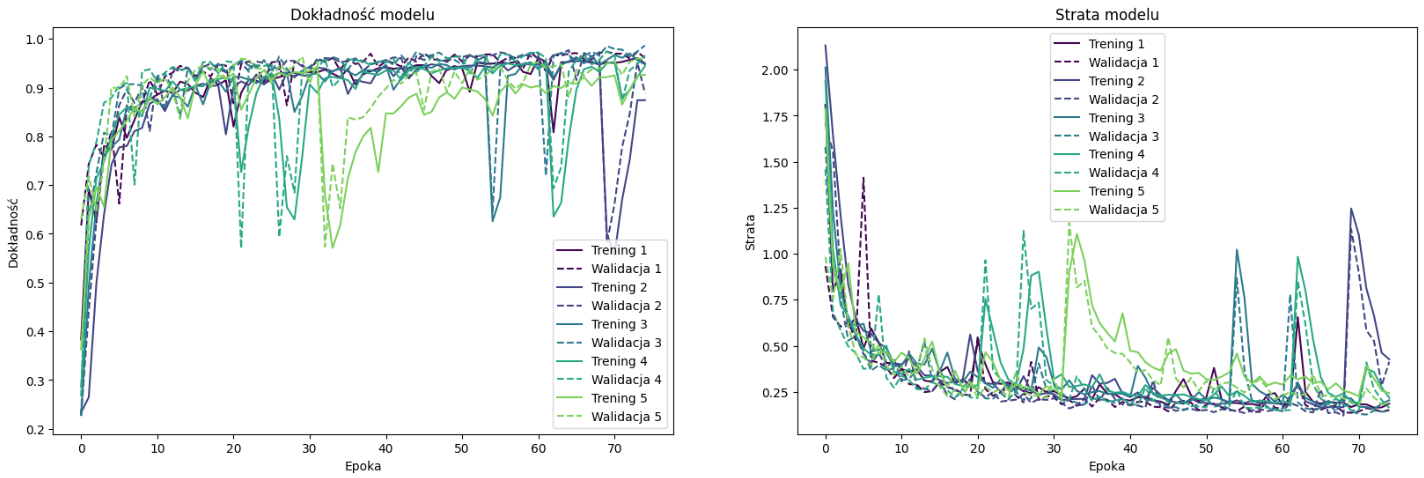
\includegraphics[height=5.5cm]{resources/tests/images/v3/crossvalid_img.png}
	\caption{Wyniki testów dla modelu z walidacją krzyżową i losową krzywizną wierzchołków}
	\label{Fig:tests-cv-1}
\end{figure}
\FloatBarrier

Podsumowując, ten wariant modelu generalnie uczy się poprawnie, dzięki czemu osiąga wysoką dokładność i niską stratę.
Fluktuacje jakie występują w wynikach, szczególnie na danych walidacyjnych,
sugerują jednak potencjalne problemy z generalizacją, co może być wynikiem niestabilności modelu,
przeuczenia modelu, lub trudności w rozpoznawaniu bardziej złożonych przykładów w danych walidacyjnych.

W przypadku tego modelu, zwiększenie liczby epok, nie przyniosłoby zamierzonych skutków.
Model zbyt szybko się przeucza, a więc większa liczba iteracji nie wpłynęłaby w żaden znaczący sposób na wynik.

% Została podjęta próba ograniczenia przeuczenia poprzez zwiększenie zbioru danych, zmiany liczby epok w modelu
% oraz manipulacji współczynnikami dropout i regularyzacji.
% W każdym przypadku model zwracał niezadowalające wyniki wynoszące 100\% po jednej z początkowych iteracji.

\begin{figure}[ht]
	\centering
	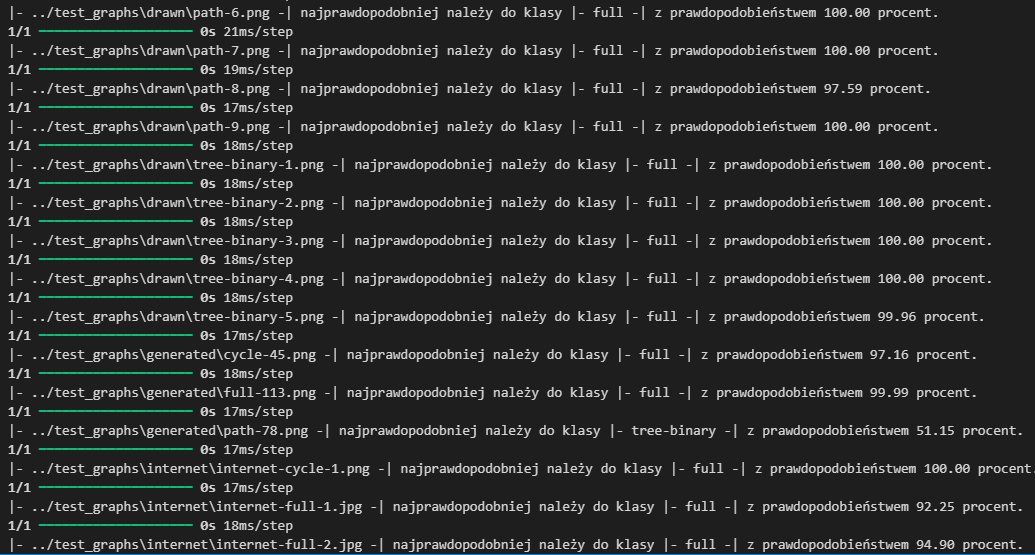
\includegraphics[height=7cm]{resources/tests/images/v3/crossvalid_txt.png}
	\caption{Klasyfikacja obrazów zewnętrznych dla modelu z walidacją krzyżową i losową krzywizną wierzchołków}
	\label{Fig:tests-cv-2}
\end{figure}
\FloatBarrier

Z powodu przeuczenia model nie radził sobie z zewnętrznymi obrazkami testowymi.
Większość grafów określił jako grafy pełne, a jedną ze scieżek jako drzewo binarne,
co nie jest zgodne ze stanem rzeczywistym.

\textbf{Zmodyfikowany model}

W celu poprawy dokładności i zapobiegnięciu przeuczenia wprowadzone
zostały następujące modyfikacje do modelu z walidacją krzyżową.
Każde z nich zostało przetestowane w osobnym modelu.
Stworzony został również jeden model ze wszystkimi połączonymi modyfikacjami. 
\begin{itemize}[label=-,labelsep=0.4cm,leftmargin=0.6cm]
    \item Zmieniono liczbę filtrów w warstwach Conv2D z 32 w każdej warstwie, do kolejno 32, 64 oraz 128.
		Jednocześnie zwiększono parametr Dropout z 0,2 do 0,5.
    \item Zastosowano Batch Normalization pomiędzy warstwami modelu - konkretnie po każdej warstwie Conv2D.
    \item Wprowadzenie augmentacji danych przed budową modelu, która wprowadza więcej wariacji do zbioru treningowego,
		w celu poprawy zdolności generalizacyjnych.
		Wykorzystano również GPU w procesie prefetchingu i cachingu zbiorów danych, by przypsieszyć przetwarzanie danych.
	\item Skorzystanie z wywołania zwrotnego, które zmniejsza szybkość uczenia.
		W przypadku stagnacji dokładności w procesie przechodzenia przez kolejne epoki uczenia modelu
		może pomóc w lepszej konwergencji modelu.
\end{itemize}

\textbf{Zmodyfikowany model - Conv2D i Dropout}

Wszystkie przebiegi walidacji krzyżowej osiągają wysoką dokładność po kilku pierwszych epokach.
Model bardzo szybko uczy się rozpoznawać wzorce.
Walidacja również osiąga zadoalające wyniki, tj. około 90\%. Może to wskazywać na poprawną generalizację do nowych danych.
Występuje jednak niewielka niesabilność, występująca pomiędzy epokami,
co widać po gwałtownych spadkach i wzrostach dokładności walidacji.

Strata na zbiorze treningowym i walidacyjnym systematycznie maleje z kolejnymi epokami,
co może wskazywać na dobre dopasowanie do danych treningowych.
Zauważalnym problemem jest jednak spora fluktuacja obu wskaźników.
Model może napotykać trudności z pewnymi próbkami w zbiorze danych walidacyjnych. 

\begin{figure}[ht]
	\centering
	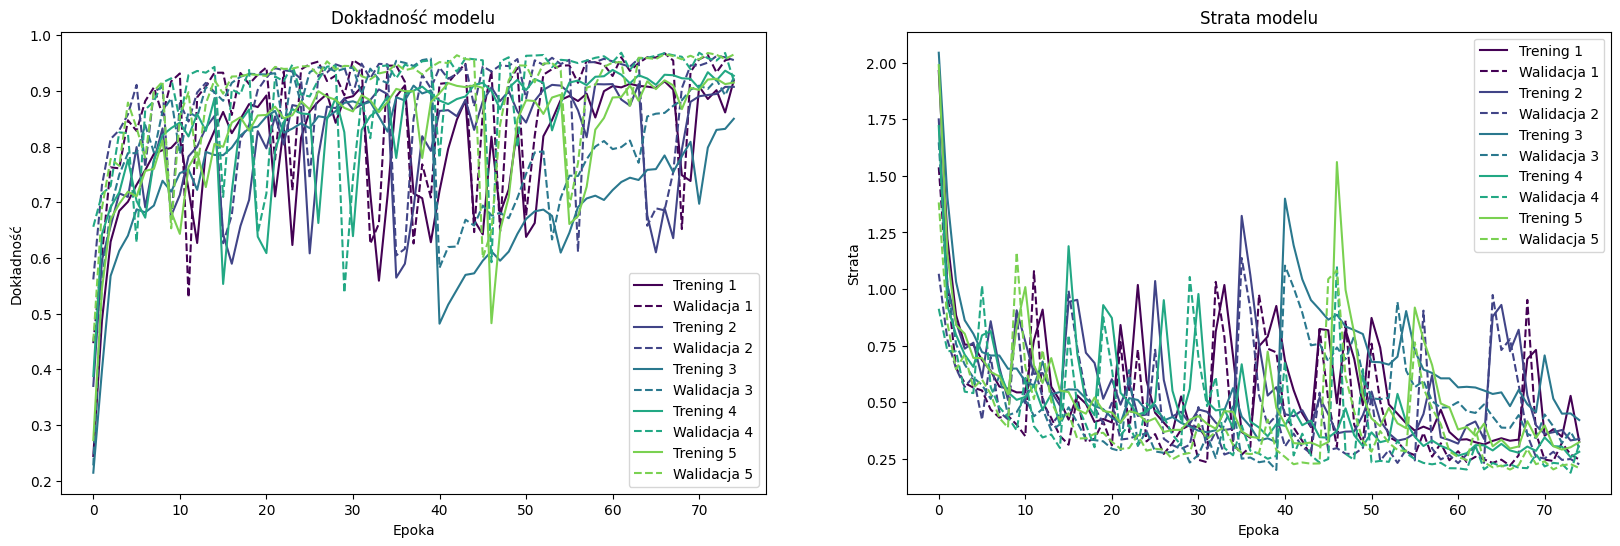
\includegraphics[height=5.5cm]{resources/tests/images/v4/crossvalid_1_img.png}
	\caption{Wyniki testów dla zmodyfikowanego modelu z walidacją krzyżową i losową krzywizną wierzchołków}
	\label{Fig:tests-cv-1}
\end{figure}
\FloatBarrier

Modfyikacja modelu wydaje się osiągać zamierzone skutki,
ponieważ model wykazuje lepszą zdolność uczenia z danych treningowych
oraz osiąga wysoką dokładność na danych walidacyjnych.
Model może być jednak wrażliwy na trudniejsze przypadki ze zbioru danych walidacyjnych,
zważając na wahania wskaźników.

\begin{figure}[ht]
	\centering
	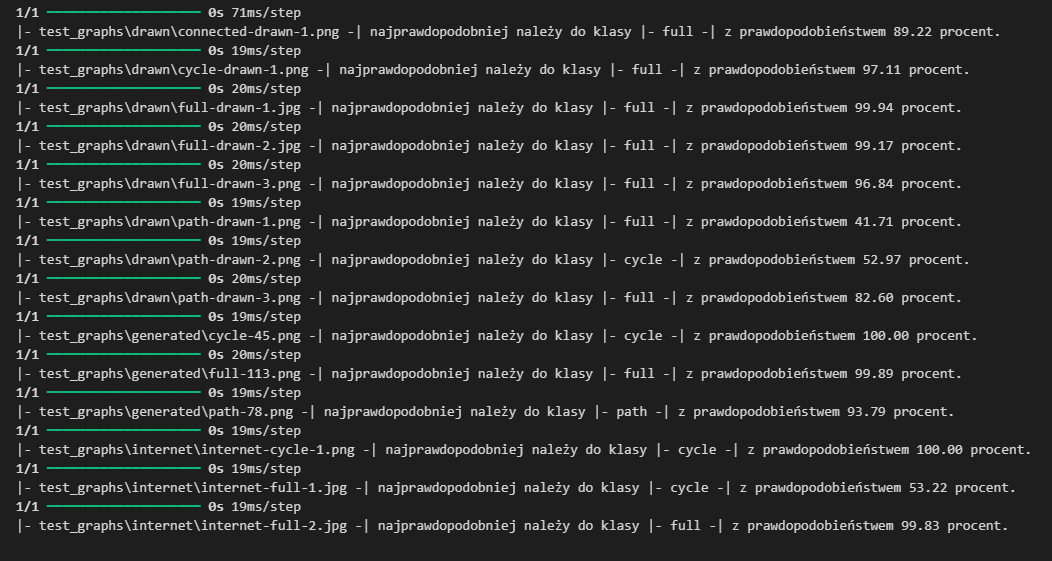
\includegraphics[height=5.5cm]{resources/tests/images/v4/crossvalid_1_txt.png}
	\caption{Wyniki testów dla zmodyfikowanego modelu z walidacją krzyżową i losową krzywizną wierzchołków}
	\label{Fig:tests-cv-1}
\end{figure}
\FloatBarrier

Model poprawnie sklasyfikował 9 rysunków grafów,
co jest znacznym polepszeniem w stosunku do początkowego modelu z zastosowaną walidacją krzyżową.

\textbf{Zmodyfikowany model połączony}

Dokładność dla wszystkich przebiegów stopniowo wzrasta wraz z liczbą epok
i osiąga wysoki poziom, bo powyżej 80\%, pod koniec treningu.
W przypadku walidacji jednak, wyniki nie są zadowalające, a wrecz bardzo niestabilne.
Przez większość przebiegów uczenia utrzymuje się na niskim poziomie,
co może sugerować problemy z generalizacją danych.

Strata treningowa maleje w większości przebiegów, co jest spodziewane podczas uczenia.
Widać jednak pewne fluktuacje, świadczące o problemach z konwergencją.
Dla straty walidacyjnej można zaobserować wielką niestabilność - osiąga bardzo wysokie wartości,
nawet rzędu kilku tysięcy, jak również bardzo niskie, bliskie zeru.

\begin{figure}[ht]
	\centering
	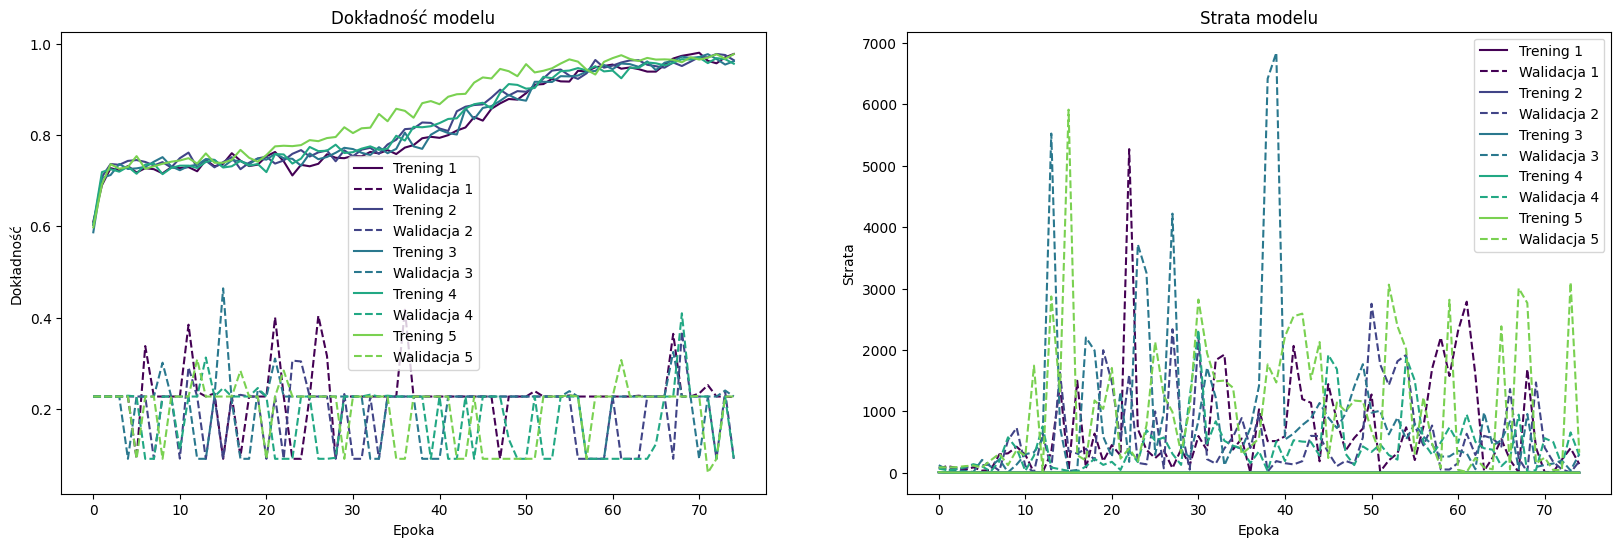
\includegraphics[height=5.5cm]{resources/tests/images/v4/crossvalid_img.png}
	\caption{Wyniki testów dla zmodyfikowanego modelu z walidacją krzyżową i losową krzywizną wierzchołków}
	\label{Fig:tests-cv-1}
\end{figure}
\FloatBarrier

Ogólne wnioski jakie można wyciągnąć z procesu uczenia tego modelu,
są takie, że model kompletnie nie radzi sobie z danymi walidacyjnymi.
Model ewidentnie przeucza się na danych treningowych,
podczas gdy jego wydajność na zbiorze walidacyjnym jest bardzo słaba.
Zastosowanie wszystkich zaproponowanych technik na raz,
nie osiągnęło zamierzonego skutku. 

\begin{figure}[ht]
	\centering
	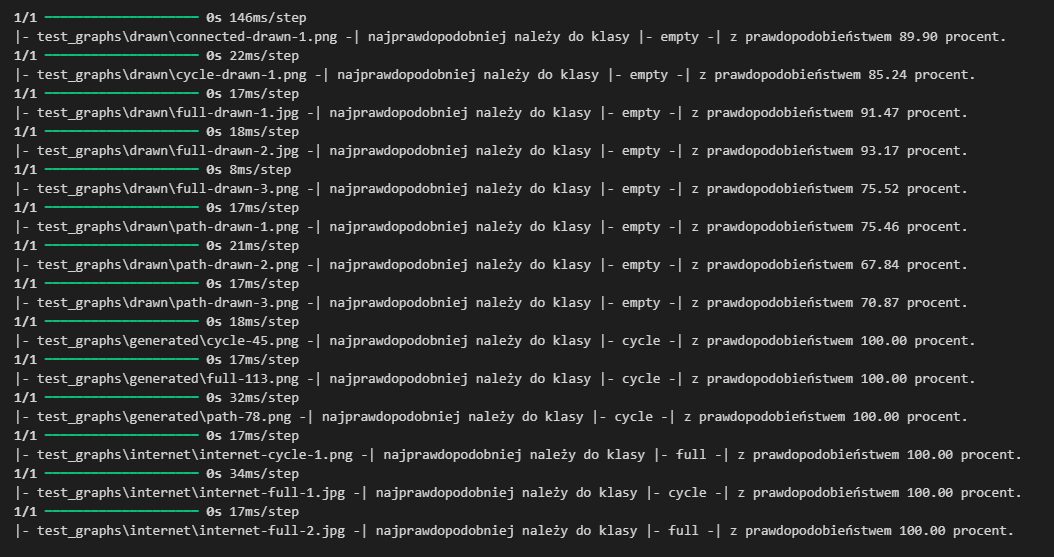
\includegraphics[height=7cm]{resources/tests/images/v4/crossvalid_txt.png}
	\caption{Klasyfikacja obrazów zewnętrznych dla zmodyfikowanego modelu z walidacją krzyżową i losową krzywizną wierzchołków}
	\label{Fig:tests-cv-2}
\end{figure}
\FloatBarrier

Model poprawnie wskazał klasy tylko dwóch grafów testowych, co jest znacznie poniżej oczekiwanych rezultatów.